\documentclass{beamer}% {{{
\usepackage{amssymb, latexsym, amsmath, graphics, fullpage, epsfig, amsthm, relsize, pgf, tikz, amsfonts, makeidx, latexsym, ifthen, hyperref, calc}
%\usepackage{eucal} this is a different font than \mathcal{•}
\usetikzlibrary{arrows}
%\newtheorem{theorem}{Theorem}[section]
\newtheorem{remark}{Remark}[section]
%\newtheorem{corollary}{Corollary}
%\newtheorem{lemma}{Lemma}[section]
\newtheorem{assumptions}{Assumptions}[section]
\newtheorem{proposition}{Proposition}
%\newtheorem{definition}{Definition}
\newtheorem{notation}{Notation}
\usepackage{mathrsfs}
%\usepackage[shortlabels]{enumitem}
\usepackage{tikz}
\usepackage{amsmath}
\usetikzlibrary{arrows}
\usetikzlibrary{shadows.blur}
\usepackage{pgfplots}
\usepackage{mwe} % For dummy images
\usepackage{subcaption}
\usepackage{multirow}
\usepackage{dcolumn}
\newcolumntype{2}{D{.}{}{2.0}}
\usepackage{multicol}
\numberwithin{equation}{section}

\newcommand{\lip}{\textup{Lip}_b}
\newcommand{\liph}{\text{Lip}_{\hat\rho}}
\newcommand{\R}{\mathbb{R}}
\newcommand{\E}{\mathbb{E}}
\newcommand{\Norm}[1]{\left\|  #1   \right\|}
\newcommand{\ud}{\ensuremath{\mathrm{d} }}

%\usepackage{lipsum}%% a garbage package you don't need except to create examples.
%\usepackage{fancyhdr}
%\pagestyle{fancy}
%\lhead{\Huge Version A}
%\rhead{\thepage}
%\cfoot{}
%\renewcommand{\headrulewidth}{0pt}



\setbeamersize{text margin left=2mm,text margin right=2mm}

\usepackage{tikz}
\usepackage{pgfplots}
\pgfplotsset{compat=newest}
\usetikzlibrary{decorations.markings}

\allowdisplaybreaks


\defbeamertemplate{footline}{higher page number}
{%
	\hfill%
	\usebeamercolor[fg]{page number in head/foot}%
	\usebeamerfont{page number in head/foot}%
	\insertframenumber\,/\,\inserttotalframenumber\kern0em\vskip20pt / 24%
}
\setbeamertemplate{footline}[page number]
% \usefoottemplate{\hfill \insertframenumber{} / 24}

% }}}
%Information to be included in the title page:
\title[About Beamer] %optional
{The Interpolated Stochastic Heat and Wave Equation: Solvability and Exact Moment Asymptotics}

\author[Arthur, Doe] % (optional, for multiple authors)
{Nicholas Eisenberg}

\pgfdeclareimage[height=1.2cm]{AU}{figs/AU.png}
\institute[Auburn University]
{
\pgfuseimage{AU}\\[3em]
 \vspace{2em}
}

\date[VLC 2021] % (optional)
{ \small Special Session on \\
	{\it Stochastic Analysis and Applications}\\[1em]
	Fall Southeastern Sectional Meeting\\[0.5em]
	November 20-21, 2021}

\logo{\includegraphics[height=1cm]{overleaf-logo}}
\thispagestyle{empty}

\begin{document}


	\frame{\titlepage}
	\setcounter{page}{1}

	\begin{frame}[t]
		\frametitle{The Interpolated Stochastic Heat and Wave Equation.}

		\begin{equation*}
		\begin{cases}
		\left(\partial^b_t + \frac{\nu}{2}(-\Delta)^{a/2}\right)\: u(t,x) = I^r_t \left[\sqrt{\theta}\: u(t,x)\: \dot W(x) \right] & \text{$x\in \R^d$, $t>0$}, \\
		u(0,\cdot) = 1                                                                                                             & b \in (0,1],               \\
		u(0,\cdot) = 1, \quad \partial_t u(0,\cdot) = 0                                                                            & b \in (1,2),
		\end{cases}
		\end{equation*}


		\begin{itemize}
			\item $\partial^b_t$ is the Caputo fractional derivative
			\item $(-\Delta)^{a/2}$ is the fractional Laplacian of order $a \in (0,2]$
			\item $I^r_t$ is the Riemann-Liouville fractional integral of order $r \ge 0$
			\item $W = \{ W(\phi) : \phi \in \mathcal{D}(\R^d) \}$ is a centered Gaussian and time-independent noise
		\end{itemize}

	\end{frame}

	\begin{frame}[t]
		\frametitle{Case of $b=a=2$ and $r=0$ and the Riesz kernel noise.}

		\begin{equation*}
		\begin{cases}
		\frac{\partial^2 u}{\partial t^2}(t,x) = \Delta u(t,x) + \sqrt{\theta}\: u(t,x)\: \dot W(x) & \text{$x\in \R^d$, $t>0$}, \\

		u(0,\cdot) = 1, \quad \partial_t u(0,\cdot) = 0                                                                            & b \in (1,2),
		\end{cases}
		\end{equation*}

		\begin{theorem}[Balan, Chen, L. and Chen, X.]
			Suppose $\mu(\ud x) = |x|^{-d+\alpha} \ud x$ and that $0 < \alpha < d \le 3$. Let $t_p:=(p-1)^{1/(4-\alpha)}t$. Then the following moment asymptotic holds:
			\[
			\lim_{t_p \to \infty} t_p^{-\frac{4-\alpha}{3-\alpha}} \log \Norm{u(t,x)}_p = \theta^{\frac{1}{3-\alpha}} 2^{\frac{-\alpha}{2(3-\alpha)}} \frac{3- \alpha}{2} \left( \frac{2 \mathcal{M}^{1/2}}{4-\alpha} \right)^{\frac{4-\alpha}{3-\alpha}}.
			\]
			In addition by fixing $p\ge 2$, we get that
			\[
			\lim_{t \to \infty} t^{-\frac{4-\alpha}{3-\alpha}} \log \mathbb{E}|u(t,x)|^p =p(p-1)^{\frac{1}{3-\alpha}} \theta^{\frac{1}{3-\alpha}} 2^{\frac{-\alpha}{2(3-\alpha)}} \frac{3- \alpha}{2} \left( \frac{2 \mathcal{M}^{1/2}}{4-\alpha} \right)^{\frac{4-\alpha}{3-\alpha}}.
			\]
		\end{theorem}
	\end{frame}

	\begin{frame}[t]
		\frametitle{Gaussian Processes}

		A Gaussian Processes, $G := \{G_t : t \in T\}$ is a stochastic process such that for and finite set of $t_1,...,t_n \in T$, the random vector $(G(t_1),...,G(t_n))$ follows a $n$-dimensional Gaussian distribution. The processes $G$ is uniquely determined by
		\begin{enumerate}
			\item $\mu(t) = \E(G(t))$
			\item $C(s,t) = \E(G(t)G(s))$
		\end{enumerate}

		\begin{theorem}[Important]
			The space of all symmetric and non-negative definite functions, $f(s,t)$, on $T\times T$ matches the space of all covariance functions of all Gaussian processes on $T$. Thus, given a non-negative definite function on $T \times T$ then there exists a Gaussian Processes that possesses this covariance function.
		\end{theorem}
	\end{frame}

	\begin{frame}[t]
		\frametitle{The noise, $\dot{W}$.}
		We start with a nonnegative and nonnegative definite tempered measure $\Gamma$ with density $\gamma$,
		\[
		\Gamma(\ud x) = \gamma(x) \ud x.
		\]
		Bochner's theorem guarantees the existence of a measure $\mu$, the spectral measure, defined through the following:
		\[
		\int_{\R^d}\Gamma(\ud x) \phi(x) = \int_{\R^d} \mathcal{F}\phi(\xi) \mu(\ud \xi) \qquad \phi \in \mathscr{S}(\R^d).
		\]

	We now define a functional on $C_0^{\infty}(\R^d)$.
		\[
			C(\phi,\psi) =  \int_{\R^d} \mathcal{F}\phi(\xi) \overline{\mathcal{F}\psi(\xi)} \mu (\ud \xi)
		\]
	\end{frame}

\begin{frame}[t]
\frametitle{The noise, $\dot{W}$.}
Recalling the theorem mentioned above, we have a zero mean Gaussian processes,$W=\{ W(\phi) : \phi \in C_0^{\infty}, \; \phi(x)\}$, with covariance given by $C(\cdot,\cdot)$. In other words,
	\begin{align*}
		\mathbb{E}(W(\phi)W(\psi)) &= \int_{\R^d} \mathcal{F}\phi(\xi) \overline{\mathcal{F}\psi(\xi)} \mu (\ud \xi)
		\\ &= \int_{\R^{2d}} \phi(x)\psi(y) \gamma(x-y) \ud x \ud y.
	\end{align*}
When $\mu$ has a density, we denote it as $\varphi(x)$.
	\end{frame}

	\begin{frame}
		\frametitle{Spatially Correlated Versus White Verses Independent}
\begin{itemize}
	\item Correlated: \[\mathbb{E}(W(\phi)W(\psi))=\int_{\R^{2d}} \phi(x)\psi(y) \gamma(x-y) \ud x \ud y.\]
	\item White:
		\begin{align*}
			\mathbb{E}(W(\phi)W(\psi))&=\int_{\R^{2d}} \phi(x)\psi(y) \delta_0(x-y) \ud x \ud y
			\\&= \int_{\R^{2d}} \phi(x)\psi(x) \ud x
		\end{align*}
		and informally we may think that $\mathbb{E}(\dot{W}(x)\dot{W}(y)) = \delta_0(x-y)$.
	\item Independent: \[ \mathbb{E}(W(\phi)W(\psi)) = \mathbb{E}(W(\phi))\mathbb{E}(W(\psi)) =0 \quad \text{for all } \phi, \psi.\]
\end{itemize}
	\end{frame}

	\begin{frame}[t]
		\frametitle{The noise, $\dot{W}$.}
		\begin{itemize}
			\item Let $k \in \{1,\cdots,d\}$
			\item Partition the $d$-coordinates of $x=(x_1,\cdots,x_d)$ into $k$ distinct groups of size $d_i$ so that $d_1 + \cdots d_k =d$
			\item $x_{(i)} = (x_{i_1},\cdots, x_{i_{d_i}})$ denotes the coordinates of the $i^{th}$ partition.
			\item Choose $\alpha_i \in (0,d_i)$ and denote $\alpha = \sum_{i=1}^k\alpha_i$
		\end{itemize}

		We consider the following Riesz-type spatial correlation function and its spectral density:
		\[
		\gamma(x) = \prod_{i=1}^k |x_{(i)}|^{-\alpha_i} \quad \varphi(\xi) = \prod_{i=1}^k C_{\alpha_i,d_i} |{\xi}_{(i)}|^{d_i-\alpha_i}.
		\]

		Note that when $k=1$, the above reduces to the Riesz kernel.
	\end{frame}

	\begin{frame}[t]
		\frametitle{The fundamental solution.}
		\[
		\begin{cases}
		\left(\partial^b_t + \frac{\nu}{2}(-\Delta)^{a/2}\right)\: u(t,x) = I^r_t \left[f(t,x)\right] & \text{$x\in \R^d$, $t>0$}, \\
		u(0,\cdot) = 1                                                                                                             & b \in (0,1],               \\
		u(0,\cdot) = 1, \quad \partial_t u(0,\cdot) = 0                                                                            & b \in (1,2),
		\end{cases}
		\]

		When $f(t,x)$ is a deterministic function, the fundamental solution given through the triple
		\[
		\{ Z_{a,b,r,\nu,d}(t,x),   Z^*_{a,b,r,\nu,d}(t,x), Y_{a,b,r,\nu,d}(t,x)\}
		\]
		where each member is defined explicitly through the Fox-H function. We have for $b \in (0,1]$ and $b \in (1,2)$ respectively that
		\[ u(t,x) =
		\begin{cases}
		(Z(t,\cdot)*u(0,\cdot))(x) + (Y\star f)(t,x)
		\\ 	(Z^*(t,\cdot)*u(0,\cdot))(x) + (Z(t,\cdot)*\partial_tu(0,\cdot))(x) + (Y\star f)(t,x).
		\end{cases}
		\]


	\end{frame}

	\begin{frame}[t]
		\frametitle{Assumption on $G$}
		We need to make an assumption that $G(t,x) = Y_{a,b,r,\nu,d}(t,x)$ is nonnegative. This is the case under any of the following:
		\begin{itemize}
			\item $d \ge 1$, $b\in(0,1]$, $a\in(0,2]$, $r\ge0$;
			% \item $d \ge 1$, $b=1$, $a\in (0,2]$, $r=0$ or $r>1$;
			\item $1\le d \le 3$, $1<b<a\le 2$, $r>0$;
			\item $1 \le d \le 3$, $1 < b=a < 2$, $r > \dfrac{d+3}{2}-b$.
		\end{itemize}
		\begin{figure}[htpb]
			\centering
			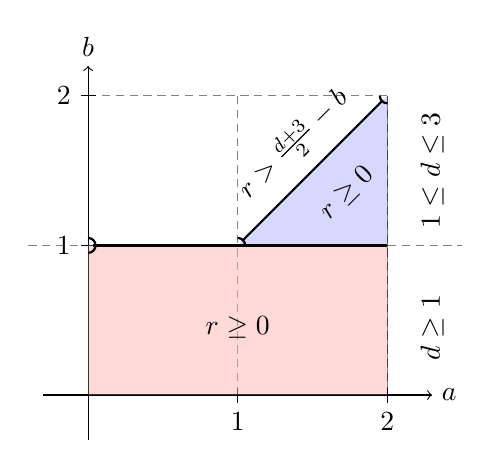
\begin{tikzpicture}[scale=1.9]
			\draw [->] (-0.3,0) -- (2.3,0) node [right] {$a$};
			\draw [->] (0,-0.3) -- (0,2.2) node [above] {$b$};
			\draw [densely dashed,gray] (1,0) -- (1,2) (2,0) -- (2,2) (-0.4,1) -- (2.5,1) (0,2) -- (2,2);
			\draw (1,0.05) -- (1,-0.05) node [below] {$1$};
			\draw (2,0.05) -- (2,-0.05) node [below] {$2$};
			\draw (0.05,1) -- (-0.05,1) node [left] {$1$};
			\draw (0.05,2) -- (-0.05,2) node [left] {$2$};
			\filldraw [fill=red!30, opacity=0.5] (0,0) rectangle (2,1);
			\filldraw [fill=blue!30, opacity=0.5] (1,1) -- (2,1) -- (2,2);
			\draw [thick] (1.03,1.03) -- (1.97,1.97);
			\draw [thick] ([shift=(0:0.05)]1,1) arc (0:90:0.05);
			\draw [thick] ([shift=(180:0.05)]2,2) arc (180:270:0.05);
			\node at (2.3,1.5) [rotate=90, anchor=center] {$1\le d\le 3$};
			\node at (2.3,0.45)[rotate=90, anchor=center] {$d\ge 1$};
			\draw [thick] (0.03,1) -- (2,1);
			\draw [thick] ([shift=(-90:0.05)]0,1) arc (-90:90:0.05);
			\node at (1.73,1.35) [rotate=45, anchor=center] {$r\ge 0$};
			\node at (1,0.45) {$r\ge 0$};
			% \node at (1,0.9) {$r=0$ or $r>1$};
			\node at (1.5,1.55) [rotate=45,anchor=south] {$r>\frac{d+3}{2}-b$};
			\end{tikzpicture}
		\end{figure}
	\end{frame}

	\begin{frame}[t]
		\frametitle{Mild solution}
		Considering the constant 1 initial condition, it can be shown the solution to the homogeneous equation is equal to $1$.
		\begin{definition}
			Let $G(t,x) = Y_{a,b,r,\nu,d}(t,x)$. For $T > 0$, a random field $u=\{u(t,x): t \in (0,T), x \in \R^d \} $ is called a \textit{mild solution} if $G(t-s,x-\cdot)u(s,\cdot)1_{\{s<t\}}$ is Skorohod integrable and the following holds almost surely:
		\end{definition}
		\[
		u(t,x) = 1 + \sqrt{\theta} \int_0^t \left(\int_{\R^d} G(t-s,x-y)u(s,y)W(\delta y)\right) \ud s.
		\]

		\begin{itemize}
			\item \textit{Global Solution:} $\Norm{u(t,x)}_p < \infty$ for any $t>0$ and $x \in \R^d$.
			\item \textit{Local Solution:} If there exists $0 < T_1 \le T_2 < \infty$ such that $\Norm{u(t,x)}_2 < \infty$ when $0<t<T_1$ and $\Norm{u(t,x)}_2 $ D.N.E. for $t> T_2$.
		\end{itemize}
	\end{frame}


	\begin{frame}[t]
		\frametitle{Wiener Chaos Expansion:}
		If $t=t_{n+1}$ and $x=x_{n+1}$, then a Picard iteration scheme will suggest that for
		\[
		f_n(x_1, \cdots , x_n; x, t) = \int_0^t\int_0^{t_n}\cdots \int_0^{t_2} \prod_{k=1}^n G(t_{k+1}-t_k,x_{k+1}-x_k) \ud t_1 \cdots \ud t_n,
		\]
		the solution can be written as
		\begin{equation}\label{E:WC}
		u(t,x) = 1 + \sum_{k=1}^\infty \theta^{k/2} I_k(f_k(\cdot,x,t)), \quad (t,x)\in (0,T)\times \R^d.
		\end{equation}
		This further suggests
		\begin{equation}\label{E:2Mom}
		\mathbb{E}(u(t,x)^2) = \sum_{k=0}^\infty \theta^{k} \Norm{f_k(\cdot,x,t)}^2_{\mathcal{H}^{\otimes n}}, \quad (t,x)\in (0,T)\times \R^d.
		\end{equation}
	\end{frame}

	\begin{frame}[t]
		\frametitle{Theorem 3.3 (Chen and Eisenberg)}

		\begin{theorem}
			Fix any $T \in (0,\infty]$. Suppose that $f_n(\cdot,x;t) \in \mathcal{H}^{\otimes n}$ for and $t \in (0,T)$ and $x\in \R^d$. Then the SPDE in question has a unique $L^2(\Omega)$ solution on $(0,T) \times \R^d$ if and only if the series
			\[
			\sum_{k=0}^\infty \theta^{k} \Norm{f_k(\cdot,x,t)}^2_{\mathcal{H}^{\otimes n}}, \quad (t,x)\in (0,T)\times \R^d.
			\]
			converges in $L^2(\Omega)$ for any $(t,x) \in (0,T) \times \R^d$. In this case, the second moment of the solution is given by this series.
		\end{theorem}
	\end{frame}

	\begin{frame}[t]
		\frametitle{Theorem 1.6 (Chen and Eisenberg)}
		Assuming $G(t,x)$ is nonnegative and the noise has spatial correlation $\gamma(x) = \prod_{i=1}^k |x_{(i)}|^{-\alpha_i}$:
		\begin{itemize}
			\item A \textcolor{blue}{\textit{global solution}} exists provided
			\[
			0 < \alpha < \min\left( \frac{a}{b}[2(b+r) -1], 2a, d \right)
			\]
			\item Otherwise, if
			\[
			r\in \left[0,1/2\right] \qquad \text{and} \qquad
			0<\alpha = \frac{a}{b}[2(b+r)-1] \le d,
			\]
			then a \textcolor{blue}{\textit{local solution}} exists for $t \in (0,T_p))$ where
			\[
			T_p := \dfrac{\nu^{\alpha/a}}{2 \theta (p-1) \mathcal{M}_a^{(2a-\alpha)/a}}
			\]
			and the solution D.N.E. for $t > T_2$.
		\end{itemize}
	\end{frame}

	\begin{frame}[t]
		\frametitle{Example: Solvability for the SWE ($a=b=2$)}
A local solution only exists when $\alpha = 3+2r \le d \le 3$.
\begin{figure}[htb]% {{{ F:SWE
	\centering
	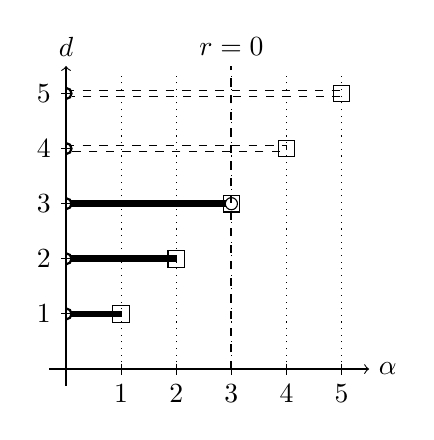
\begin{tikzpicture}[scale=0.7]
	\draw [thick,dashed] (3,0) -- (3,5.5) node [above] {$r=0$};
	\draw [->] (-0.3,0) -- (5.5,0) node [right] {$\alpha$};
	\draw [->] (0,-0.3) -- (0,5.5) node [above] {$d$};
	\foreach \x in {1,...,5}{
		\draw (\x,0.1)--++(0,-0.2) node [below] {$\x$};
		\draw (0.1,\x)--++(-0.2,0) node [left] {$\x$};
		\draw (\x,\x) + (-0.15,-0.15) rectangle +(0.15,0.15);
		\draw [thick] ([shift=(-90:0.1)]0,\x) arc (-90:90:0.1);
		\draw [thin, dotted] (\x,0) -- (\x, 5.4);
	}
	\filldraw (0, 1) + (0.1, -0.05) rectangle +(1,0.05);%\filldraw (1,1) circle (0.05);
	\filldraw (0, 2) + (0.1, -0.05) rectangle +(2,0.05);%\filldraw (2,2) circle (0.05);
	\filldraw (0, 3) + (0.1, -0.05) rectangle +(2.9,0.05);%\filldraw (3,3) circle (0.05);
	% \filldraw (0, 4) + (0.1, -0.05) rectangle +(2.9,0.05);
	% \filldraw (0, 5) + (0.1, -0.05) rectangle +(2.9,0.05);
	% \draw (2,2) circle (0.11);
	\draw (3,3) circle (0.11);
	% \draw (3,4) circle (0.11);
	% \draw (3,5) circle (0.11);
	% \draw (2, 3) + (0.1, -0.05) rectangle +(1,0.05);
	% \draw (2, 4) + (0.1, -0.05) rectangle +(2,0.05);
	\draw[dashed] (0, 5) + (0.1, -0.05) rectangle +(5,0.05);
	\draw[dashed] (0, 4) + (0.1, -0.05) rectangle +(4,0.05);
	\end{tikzpicture}
	\hspace{2em}
	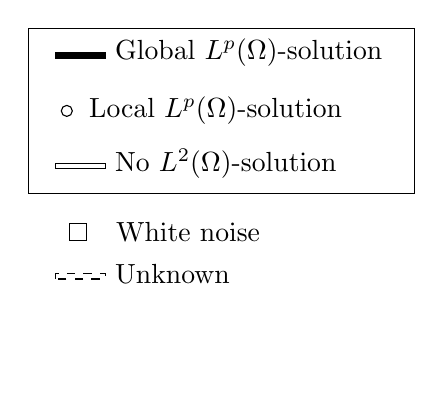
\begin{tikzpicture}[scale=0.7]
	\def\x{3.2}
	% \draw (-0.4,-1.5+\x) rectangle +(6,3);
	% \draw (0.5,0+\x) circle (0.1); \node at (3,0+\x) {Local $L^p(\Omega)$-solution};
	% \draw (0, -1+\x) + (0.1, -0.05) rectangle +(1,0.05) node [right] {No $L^2(\Omega)$-solution};
	% \draw (0.5, 1) + (-0.15,-0.15) rectangle +(0.15,0.15); \node at (2.5,1) {White noise};
	\draw[dashed] (0, -3+\x) + (0.1, -0.05) rectangle +(1,0.05) node [right] {Unknown};
	\draw (-0.4,-1.5+\x) rectangle +(7,3);
	\filldraw (0, 1+\x) + (0.1, -0.05) rectangle +(1,0.05) node [right] {Global $L^p(\Omega)$-solution};
	\draw (0.3,0+\x) circle (0.1); \node at (3,0+\x) {Local $L^p(\Omega)$-solution};
	\draw (0, -1+\x) + (0.1, -0.05) rectangle +(1,0.05) node [right] {No $L^2(\Omega)$-solution};
	\draw (0.5, 1) + (-0.15,-0.15) rectangle +(0.15,0.15); \node at (2.5,1) {White noise};
	\draw[white] (0,-1.5) circle (0.01);
	\end{tikzpicture}
\end{figure}% }}}
By replacing $\nu=2$ in the following, we recover (1.12) Balan, Chen and Chen:
	\[
		T_p=	\frac{\nu^{3 / 2}}{2\theta (p-1) \sqrt{\mathcal{M}_{2,3}(\delta_0)}},  \quad p\ge 2
	\]



	\end{frame}

	\begin{frame}[t]
		\frametitle{Example: Solvability for the SHE ($a=2$ and  $b=1$)}
			By setting $a=2$, $b=1$ and $r=0$, we obtain the following condition for existence of a local solution: $\alpha = 2 \le d.$
	\begin{columns}
		\begin{column}{0.5\textwidth}
		\begin{figure}[htpb]% {{{ F:SHE
			\centering
			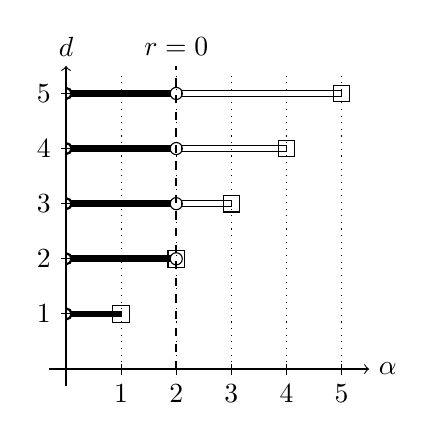
\begin{tikzpicture}[scale=0.7]
			\draw [thick,dashed] (2,0) -- (2,5.5) node [above] {$r=0$};
			\draw [->] (-0.3,0) -- (5.5,0) node [right] {$\alpha$};
			\draw [->] (0,-0.3) -- (0,5.5) node [above] {$d$};
			\foreach \x in {1,...,5}{
				\draw (\x,0.1)--++(0,-0.2) node [below] {$\x$};
				\draw (0.1,\x)--++(-0.2,0) node [left] {$\x$};
				\draw (\x,\x) + (-0.15,-0.15) rectangle +(0.15,0.15);
				\draw [thick] ([shift=(-90:0.1)]0,\x) arc (-90:90:0.1);
				\draw [thin, dotted] (\x,0) -- (\x, 5.4);
			}
			\filldraw (0, 1) + (0.1, -0.05) rectangle +(1,0.05);%\filldraw (1,1) circle (0.05);
			\filldraw (0, 2) + (0.1, -0.05) rectangle +(1.9,0.05);
			\filldraw (0, 3) + (0.1, -0.05) rectangle +(1.9,0.05);
			\filldraw (0, 4) + (0.1, -0.05) rectangle +(1.9,0.05);
			\filldraw (0, 5) + (0.1, -0.05) rectangle +(1.9,0.05);
			\draw (2,2) circle (0.11);
			\draw (2,3) circle (0.11);
			\draw (2,4) circle (0.11);
			\draw (2,5) circle (0.11);
			\draw (2, 3) + (0.1, -0.05) rectangle +(1,0.05);
			\draw (2, 4) + (0.1, -0.05) rectangle +(2,0.05);
			\draw (2, 5) + (0.1, -0.05) rectangle +(3,0.05);
			\end{tikzpicture}
		\end{figure}
	\end{column}
	\begin{column}{0.5\textwidth}
		\begin{itemize}
			\item 	When $\alpha=d=2$, the critical time becomes $T_p = \dfrac{\nu}{2\theta (p-1) \mathcal{M}_{2,2}(\delta_0)}$.
			\item Theorem 4.1 (Hu) proves that an $L^2(\Omega)$ solution exists for $t<2$ but not for $t>2 \pi$.
			\item $T_2$ being precise implies $2 \le T_2 = \frac{1}{2\mathcal{M}_{2,2}(\delta_0)} \le 2\pi$
		\end{itemize}
\end{column}
\end{columns}

	\end{frame}

			\begin{frame}[t]
		\frametitle{Example: Solvability For The SHE With Fractional Laplace ($b=1$, $r=0$ and $0<a \le 2$)}
			A local solution exists when $\alpha = a \le d$. The critical time is given by $T_p = \frac{\nu}{2\theta (p-1)\mathcal{M}_{2,2}(\delta_0)}$.
	\begin{figure}[htpb]% {{{ F:Stable
		\centering
		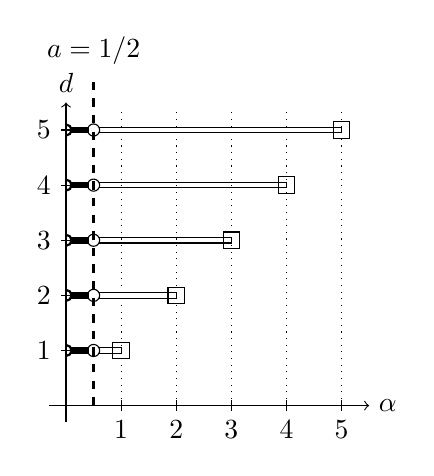
\begin{tikzpicture}[scale=0.7]
		% \draw [thick,dashed] (2,0) -- (2,5.5) node [above] {$r=0$};
		\draw [thick,dashed] (0.5,0) -- (0.5,6) node [above] {$a=1/2$};
		\draw [->] (-0.3,0) -- (5.5,0) node [right] {$\alpha$};
		\draw [->] (0,-0.3) -- (0,5.5) node [above] {$d$};
		\foreach \x in {1,...,5}{
			\draw (\x,0.1)--++(0,-0.2) node [below] {$\x$};
			\draw (0.1,\x)--++(-0.2,0) node [left] {$\x$};
			\draw (\x,\x) + (-0.15,-0.15) rectangle +(0.15,0.15);
			\draw [thick] ([shift=(-90:0.1)]0,\x) arc (-90:90:0.1);
			\draw [thin, dotted] (\x,0) -- (\x, 5.4);
		}
		\filldraw (0, 1) + (0.1, -0.05) rectangle +(0.4,0.05);
		\filldraw (0, 2) + (0.1, -0.05) rectangle +(0.4,0.05);
		\filldraw (0, 3) + (0.1, -0.05) rectangle +(0.4,0.05);
		\filldraw (0, 4) + (0.1, -0.05) rectangle +(0.4,0.05);
		\filldraw (0, 5) + (0.1, -0.05) rectangle +(0.4,0.05);
		\draw (0.5,1) circle (0.11);
		\draw (0.5,2) circle (0.11);
		\draw (0.5,3) circle (0.11);
		\draw (0.5,4) circle (0.11);
		\draw (0.5,5) circle (0.11);
		\draw (0.5,1) + (0.1, -0.05) rectangle +(0.5,0.05);
		\draw (0.5,2) + (0.1, -0.05) rectangle +(1.5,0.05);
		\draw (0.5,3) + (0.1, -0.05) rectangle +(2.5,0.05);
		\draw (0.5,4) + (0.1, -0.05) rectangle +(3.5,0.05);
		\draw (0.5,5) + (0.1, -0.05) rectangle +(4.5,0.05);
		\end{tikzpicture}
		\qquad
		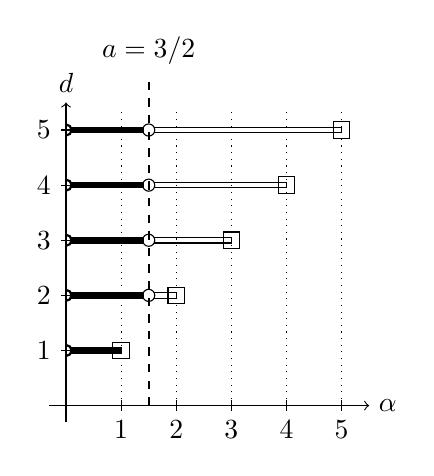
\begin{tikzpicture}[scale=0.7]
		\draw [thick,dashed] (1.5,0) -- (1.5,6) node [above] {$a=3/2$};
		% \draw [thick,dashed] (0.5,0) -- (0.5,5.5) node [above] {$r=0$};
		\draw [->] (-0.3,0) -- (5.5,0) node [right] {$\alpha$};
		\draw [->] (0,-0.3) -- (0,5.5) node [above] {$d$};
		\foreach \x in {1,...,5}{
			\draw (\x,0.1)--++(0,-0.2) node [below] {$\x$};
			\draw (0.1,\x)--++(-0.2,0) node [left] {$\x$};
			\draw (\x,\x) + (-0.15,-0.15) rectangle +(0.15,0.15);
			\draw [thick] ([shift=(-90:0.1)]0,\x) arc (-90:90:0.1);
			\draw [thin, dotted] (\x,0) -- (\x, 5.4);
		}
		\filldraw (0, 1) + (0.1, -0.05) rectangle +(1,0.05);%\filldraw (1,1) circle (0.05);
		\filldraw (0, 2) + (0.1, -0.05) rectangle +(1.4,0.05);%\filldraw (2,2) circle (0.05);
		\filldraw (0, 3) + (0.1, -0.05) rectangle +(1.4,0.05);
		\filldraw (0, 4) + (0.1, -0.05) rectangle +(1.4,0.05);
		\filldraw (0, 5) + (0.1, -0.05) rectangle +(1.4,0.05);
		\draw (1.5,2) circle (0.11);
		\draw (1.5,3) circle (0.11);
		\draw (1.5,4) circle (0.11);
		\draw (1.5,5) circle (0.11);
		\draw (1.5, 2) + (0.1, -0.05) rectangle +(0.5,0.05);
		\draw (1.5, 3) + (0.1, -0.05) rectangle +(1.5,0.05);
		\draw (1.5, 4) + (0.1, -0.05) rectangle +(2.5,0.05);
		\draw (1.5, 5) + (0.1, -0.05) rectangle +(3.5,0.05);
		\end{tikzpicture}

	\end{figure}% }}}
		\end{frame}

		\begin{frame}[t]
		\frametitle{The moment asymptotic}
		\begin{theorem}[Chen and Eisenberg]
			Suppose a global solution to the SPDE in question exists and $\dot{W}$ is given through the generalized Riesz kernel defined above. Then,
			\begin{align*}
			\lim_{t_p \to \infty} &  t_p^{-\beta} \log \Norm{u(t,x)}_p
			\\& =  \left(\frac{1}{2}\right)\left(\frac{2a}{2a(b+r)- b\alpha} \right)^\beta \\
			& \quad \quad \quad  \times \left(\theta\nu^{-\alpha/a} \mathcal{M}_a^{\frac{2a-\alpha}{a}}\right)^{\frac{a}{2a(b+r)-b\alpha-a}}\left(2(b+r)-\frac{b\alpha}{a}-1\right),
			\end{align*}
			where
			\begin{align}
			\label{E:beta-tp}
			\beta := \dfrac{2(b+r)-\dfrac{b\alpha}{a}}{ 2(b+r)-\dfrac{b\alpha}{a} -1 } \qquad \text{and} \qquad
			t_p   := (p-1)^{1-1/\beta} \: t.
			\end{align}
		\end{theorem}

	\end{frame}

	\begin{frame}[t]
		\frametitle{$\mathcal{M}$}
		We define
		\begin{align*}
		\mathcal{M}_{a,d}(\gamma,\theta) & := \sup_{g \in \mathcal{F}_a} \left\{ \left( \iint_{\R^{2d}} g^2(x)g^2(y) \gamma(x+y)\ud x\ud y \right)^{1/2} - \frac{\theta}{2}\: \mathcal{E}_a(g,g) \right\} \\
		& = \sup_{g \in \mathcal{F}_a} \left\{ \left\langle g^2 * g^2, \gamma \right\rangle_{L^2(\R^d)}^{1/2} - \frac{\theta}{2}\: \mathcal{E}_a(g,g) \right\},
		\end{align*}
		where
		\begin{gather}
		\mathcal{E}_a(g,g) := (2\pi)^{-d} \int_{\R^d} |\xi|^a |\mathcal{F}g(\xi)|^2 \ud \xi \quad \text{and} \\
		\mathcal{F}_a      := \left\{f\in L^2(\R^d): \: \Norm{f}_{L^2(\R^d)}=1,\: \mathcal{E}_a(f,f)<\infty \right\}.
		\end{gather}
	\end{frame}

		\begin{frame}[t]
		\frametitle{$\rho$}
		We define
					\begin{align*}
			\rho_{\nu,a}(\gamma) &= \sup_{\Norm{f}_{L^2(\R^d)} =1} \int_{\R^d} \left[ \int_{\R^d} \frac{f(x+y)f(y)}{\sqrt{1+\frac{\nu}{2}|x+y|^a } \sqrt{1+\frac{\nu}{2}|y|^a} } \ud y \right]^2 \mu(\ud x)
			\end{align*}

		\begin{theorem}[Chen and Eisenberg]
			When $\mu(\ud x) = \varphi(x) \ud x$ where $\varphi$ is the generalized Riesz kernel introduced above then,
			\begin{align*}
			\lim_{n \to \infty} \frac{1}{n} \log & \left[ \frac{1}{(n!)^2} \int_{(\R^d)^n} \left( \sum_{\sigma \in \Sigma_n} \prod_{k=1}^n \frac{1}{1+ \frac{\nu}{2}|\sum_{j=k}^n \xi_{\sigma(j)}|^a}\right)^2 \mu (\ud \vec{\xi})\right]
			\\& = \log\left( \rho_{\nu, a}\left(\gamma\right) \right).
			\end{align*}
			where $\gamma$ is the spatial correlation function.
		\end{theorem}

	\end{frame}

	\begin{frame}
		\frametitle{The Connection between $\rho$ and $\mathcal{M}$}
					\begin{theorem}[Chen and Eisenberg]
				When $\mu(\ud x) = \varphi(x) \ud x$ where $\varphi$ is the generalized Riesz kernel introduced above then,
				\[
				\rho_{\nu,a}(\gamma) = \nu^{-\alpha/a} \mathcal{M}_a^{2-(\alpha / a)}(\gamma)<\infty
				\]
			\end{theorem}
	\end{frame}

	\begin{frame}[t]
	\frametitle{$\rho$ and the SWE}
	\[
	\zeta\left([0,t_1]\times [0,t_2]\right) = \int_0^{t_1} \int_0^{t_2} | X_1(s_1) + X_2(s_2)|^{-\sigma} \ud s_1 \ud s_2
	\]
	where $X_1(t)$ and $X_2(t)$ are i.i.d. $d$-dimensional symmetric stable processes of index $ \beta = 2$,
	\[
	\mathbb{E}e^{i\lambda X_i(t)} = e^{-t|\lambda|^\beta}.
	\]

\begin{theorem}[X. Chen]
	\[
		\lim_{n \to \infty} \frac{1}{n} \log \frac{1}{(n!)^2} 	\mathbb{E}\bigg[ \zeta \big( [0,\tau_1] \times [0,\tau_2] \big)^n \bigg] = \log\big[\rho_{2,2}(\gamma)\big]
	\]
\end{theorem}
	\end{frame}


		\begin{frame}[t]
		\frametitle{$\rho$ and the SWE}
	\begin{theorem}[X. Chen]
		Suppose $\tau_1$ and $\tau_2$ are exponential random variables with mean 1. Then,
		\[
		\mathbb{E}\left[ \zeta\left([0,\tau_1] \times [0,\tau_2]\right)^n \right] = \int_{(\R^{d})^n} \left[ \sum_{\sigma \in \Sigma_n} \prod_{k=1}^n \frac{1}{ 1 + \left| \sum_{j=k}^n  \xi_{\sigma(j)} \right|^2 } \right]^2 \mu(\ud \vec{\xi})
		\]
	\end{theorem}
It can be shown that
	\begin{align*}
		\frac{1}{(n!)^2}\mathbb{E}[ \zeta ( [0,\tau_1]  &\times [0,\tau_2] )^n ]
		\\ &= \int_{(\R^d)^2} \mathcal{F}\mathcal{L}\left[\tilde{f}_n(\circ_1,\cdots\circ_n,0;\cdot)\right]^2(\xi_1, \cdots,\xi_n,1) \mu(\ud \vec{\xi})
	\end{align*}

	\end{frame}

	\begin{frame}[t]
		\frametitle{Exponential Growth of the Moments in Time}
		\begin{theorem}[Chen and Eisenberg] For $p \ge 2$ fixed, we have that
			\begin{align*}
			\lim_{t \to \infty} & t^{-\beta} \log \E\left(|u(t,x)|^p\right)
			\\&=  p(p-1)^{\frac{1}{2(b+r)-\frac{b\alpha}{a} -1}} \left(\frac{1}{2}\right)\left(\frac{2a}{2a(b+r)- b\alpha} \right)^\beta \\
			& \quad \quad \times \left(\theta\nu^{-\alpha/a} \mathcal{M}_a^{\frac{2a-\alpha}{a}}\right)^{\frac{a}{2a(b+r)-b\alpha-a}}\left(2(b+r)-\frac{b\alpha}{a}-1\right).
			\end{align*}
		\end{theorem}
From this we can deduce that $t \mapsto \mathbb{E}(|u(t,x)|^p)$ grows as fast as $\exp\left({K_1 t^\beta }\right)$, in other words, the moments will grow exponentially in time.


	\end{frame}

		\begin{frame}[t]
		\frametitle{Exponential Growth of the moments for Fixed Time}
		\begin{theorem}[Chen and Eisenberg] For $t>0$ fixed , we have that
			\begin{align*}
	\lim_{p \to \infty} &  p^{-\beta} \log \E\left(|u(t,x)|^p\right)
	\\ &=  t^\beta \left(\frac{1}{2}\right)\left(\frac{2a}{2a(b+r)- b\alpha} \right)^\beta \\
	& \quad \quad \times \left(\theta\nu^{-\alpha/a} \mathcal{M}_a^{\frac{2a-\alpha}{a}}\right)^{\frac{a}{2a(b+r)-b\alpha-a}}\left(2(b+r)-\frac{b\alpha}{a}-1\right).
	\end{align*}
			\end{theorem}
From this we can deduce that $p \mapsto \mathbb{E}(|u(t,x)|^p)$ grows as fast as $\exp\left({K_2 p^\beta }\right)$, in other words, the moments will grow exponentially in $p$ as well.

		\end{frame}

	\begin{frame}[t]
		\frametitle{Final Comments}
			Two possible future works.
				\begin{enumerate}
					\item Consider a time and spatially dependent noise. Ie, $W = \{W(\phi), \phi \in \mathcal{D}(\R \times \R^d)\}$
						\[
							\mathbb{E}(W(\phi)W(\psi)) = \int_{\R^{2}}\int_{\R^{2d}} \gamma(t-s)f(x-y)\phi(t,x)\psi(s,y) \ud x\ud y \ud t \ud s
						\]
					where $\gamma$ is the time correlation and $f$ is the spatial correlation.
					\item Under what type of convergence do we have as we vary the fractional parameters? How is the following limit taken:
						\[
							\lim_{a \to a_0, \; b \to b_0, \; r \to r_0, \; \nu \to \nu_0, \; \theta \to \theta_0} u_{a,b,r,\nu,\theta}(t,x) \to u_{a_0,b_0,r_0,\nu_0,\theta_0}(t,x).
						\]

				\end{enumerate}

	\end{frame}
\end{document}
